\section{Evaluation}
\label{sec:eval}
\paragraph{}
In order to measure the performance of Tracer, we performed a microbenchmark study using binary trees as an exemplar in-memory data structure. We performed four sets of tests for our microbenchmark study. We measured the overall time taken for the creation of nodes of a large binary tree. We also tested the overheads involved in the search, update and traversal operations. Our experiments were done on an Intel $i5$ virtual machine with a {\emph{2.5 GHz}} clock frequency. The DRAM size allocated to the virtual machine was {\emph{4GB}}. All the experimental results have been averaged over 10 different runs. 

\paragraph{}
We performed a comparative analysis and compared Tracer's overhead with the performance of an unmodified implementation in C (we call it the {\emph{vanilla C implementation}}). We also implemented a page protection mechanism, similar to the mechanism used in \cite{SSDAlloc} for tracking objects. Our primary objective behind the study was to measure the overall overhead of our memory monitoring mechanism and compare it with a page protection mechanism. The implementation of the page protection mechanism used a page buffer size of {\emph{25MB}} as suggested in \cite{SSDAlloc}.

\paragraph{Binary Tree Creation Tests}
The first test measured the overall overhead that Tracer has while monitoring the access to objects. We created trees containing 2500 to 25000 nodes. The experimental results indicate that Tracer invokes an overhead of around 20\% over the vanilla C implementation. The page protection mechanism has an overhead of three orders of magnitude (refer to Fig. \ref{fig:create}). The average time for creation of a binary tree with the vanilla C implementation is around 3.77 milliseconds, 4.5 milliseconds for Tracer and over 1 second for the page protection mechanism. One of the primary reasons for the poor performance of the page protection mechanism is the overheads involved in the eviction of an object from the page table and its subsequent insertion in the object table. This requires a system call (triggered due to access to a protected page), eviction of the page from the page buffer (overheads due to memory copy) and page materialization (requiring memory copy from the object table to the page buffer and a look up in the object table). 

\begin{figure}[!h]
\caption{Binary Tree Benchmark Results For Tree Creation}
\label{fig:create}
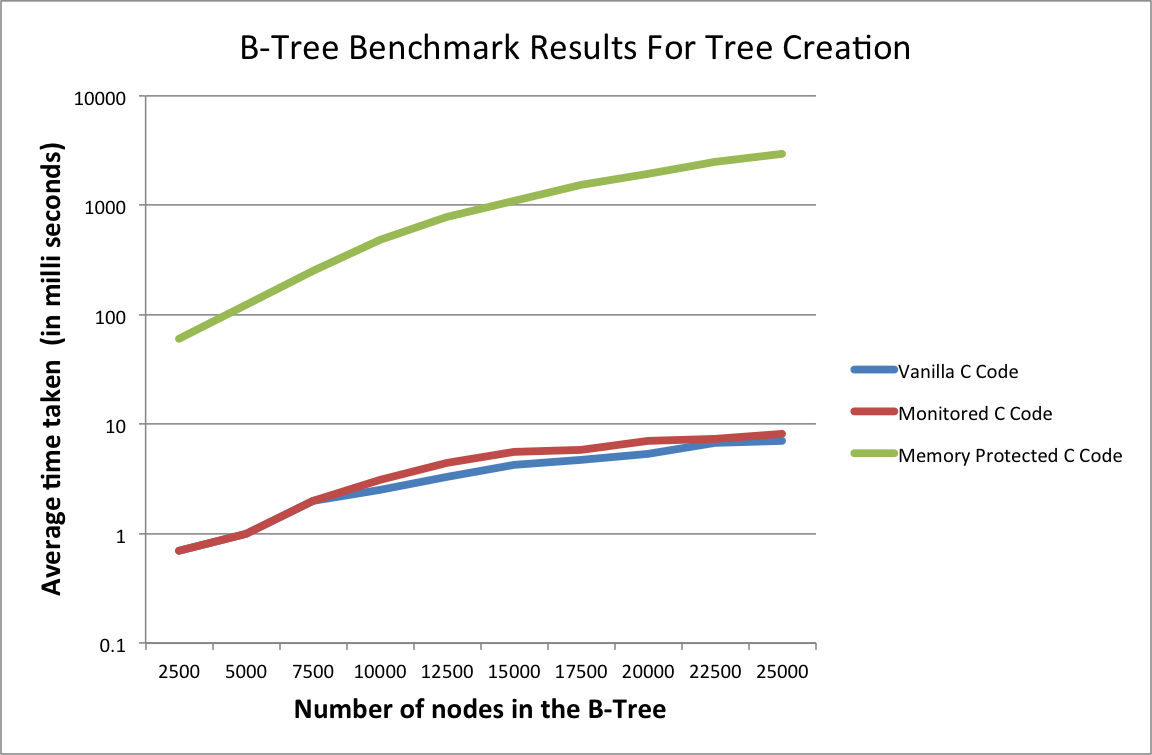
\includegraphics[scale=0.4]{./images/create.png}
\end{figure}
\begin{figure}[!h]
\caption{Binary Tree Benchmark Results For Read Workloads}
\label{fig:read}
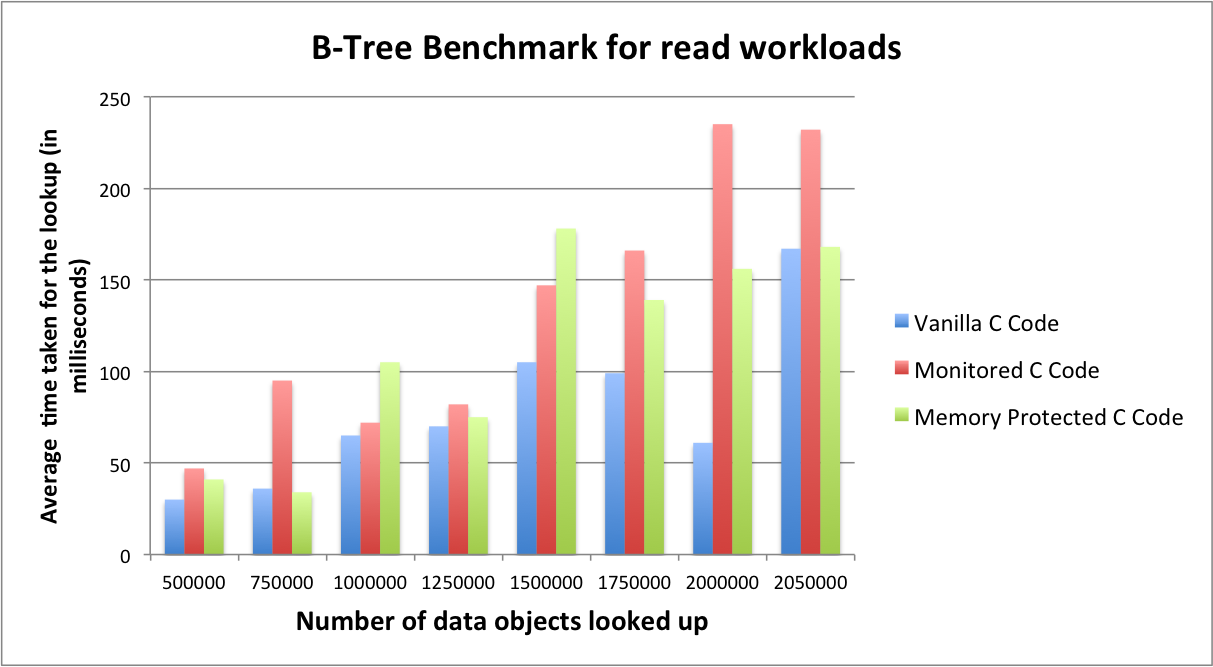
\includegraphics[scale=0.4]{./images/read.png}
\end{figure}
\begin{figure}[!h]
\caption{Binary Tree Benchmark Results For Update Workloads}
\label{fig:update}
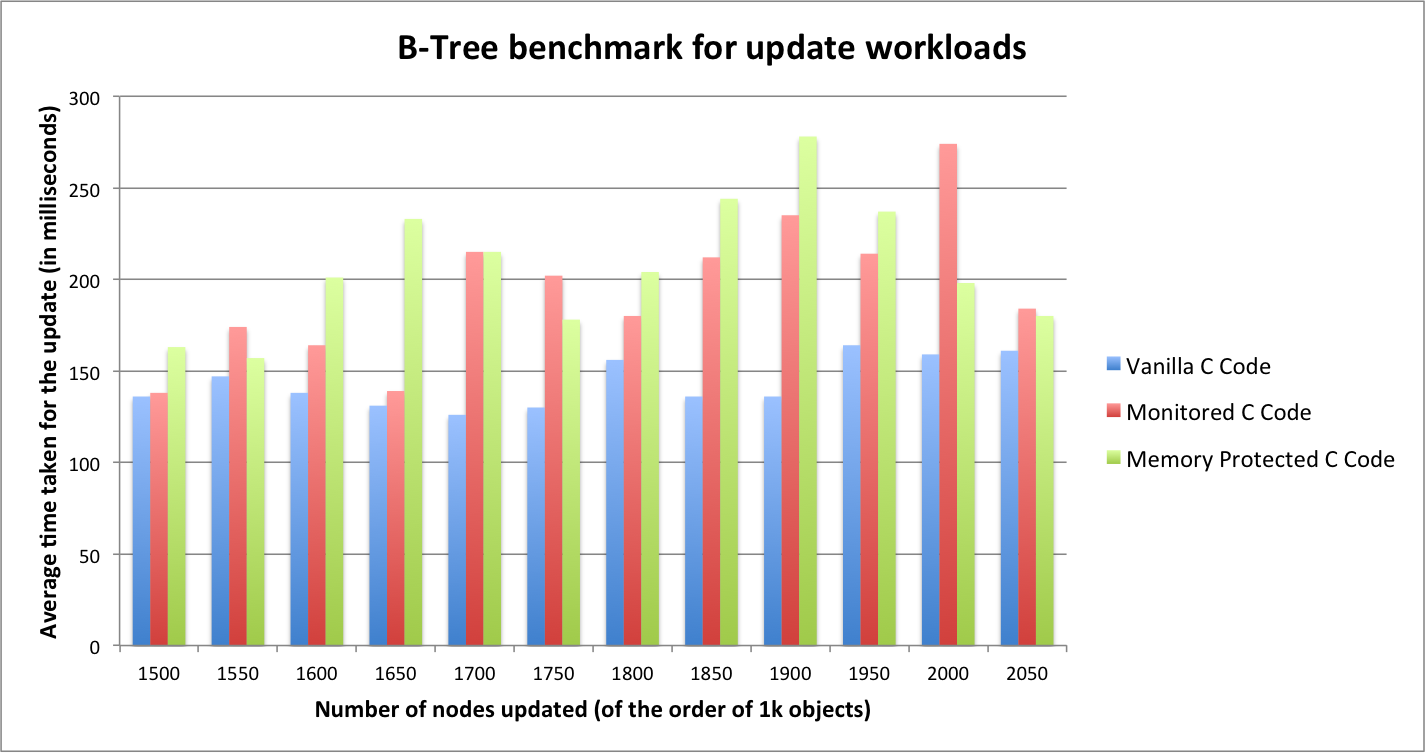
\includegraphics[scale=0.33]{./images/update.png}
\end{figure}
  

\paragraph{Binary Tree Read Tests}
The second set of tests measured the overall overhead incurred in reading a set of random objects from a Binary Tree of a fixed size (number of nodes in the binary tree was kept to 2500). For the read tests, we generated a random number of keys and search for them in a preconstructed binary tree. We varied the number of keys read from 500,000 to 2 million per experiment. Each data point is an average of 10 different experiments. Tracer has a reasonable overhead (of around $40\%$) over the vanilla C implementation, while the page protection mechanism has an overhead of $28\%$ (refer to Fig. \ref{fig:read}}). 
Tracer incurs slightly more overhead because it performs fine grained monitoring, whereas page protection mechanisms provide an approximation of the access pattern of the application. These overheads are reasonable considering the more precise information that Tracer provides the developer with.

\paragraph{Binary Tree Update Tests}
The third set of tests measured the overall overhead incurred for update intensive workloads. As in the read test, we generate a random set of key pairs. Each key pair has a source and a destination key. The source key is searched in the binary tree and its value is updated with the destination key's value. If the source key is not found in the binary tree then the update procedure returns. We varied the number of update operations from 1.5 million to 2.5 million for our tests. Tracer improves the performance of the update operations over the page protected mechanism by $6.28\%$. The overhead over the vanilla C implementation is around $35\%$. %(refer to Fig. \ref{fig:b-tree\_update.png}).
 These tests indicate that Tracer performs well in comparison to the page protection mechanism for update-heavy workloads. 

\paragraph{B-Tree Traversal Tests}
The fourth set of experiments explored the performance of tree traversals for the three different mechanisms. Tree traversals are generally observed heavily for range queries in databases. The page protected mechanism performs poorly for such workloads with over 2 orders of magnitude of overhead. 

\paragraph{}
The observation from the tree traversal and creation tests is that the page protection mechanisms perform poorly when a large number of nodes of the tree are touched. This could be explained because such an access pattern would result in a high "{\emph{object flux}}" between the page buffer and page table. The movement of an object between the page table and page buffer involves page eviction and page materialization which have high overheads. Tracer circumvents these overheads by its interception and tagged counter based approach. 
